% iaus2esa.tex -- sample pages for Proceedings IAU Symposium document class
% (based on v1.0 cca2esam.tex)
% v1.04 released 17 May 2004 by TechBooks
%% small changes and additions made by KAvdH/IAU 4 June 2004
% Copyright (2004) International Astronomical Union

\NeedsTeXFormat{LaTeX2e}

\documentclass{iaus}
\usepackage{graphicx}

\title[Galactic potential from tidal stream actions] %% give here short title %%
{Action-space clustering of tidal streams to map the Galactic potential}

\author[R.E. Sanderson, A. Helmi, \& D. Hogg]   %% give here short author list %%
{Robyn E. Sanderson$^1$, Amina Helmi $^1$,
%%  \thanks{Present address: Fluid Mech Inc., 24 The Street, Lagos, Nigeria.},
 \and David Hogg$^2$}

\affiliation{$^1$ Kapteyn Astronomical Institute, P.O. Box 800, 9700AV Groningen, Netherlands\\ email: {\tt sanderson@astro.rug.nl} \\[\affilskip]
$^2$ Center for Cosmology and Particle Physics, Department of Physics, New York University, 4 Washington Place, New York, NY  10003, USA}

\pubyear{2014}
\volume{298}  %% insert here IAU Symposium No.
\pagerange{XX -- YY}
% \date{?? and in revised form ??}
\setcounter{page}{1}
\jname{IAUS\,298 Setting the scene for Gaia and LAMOST}
\editors{S. Feltzing, G. Zhao, N.\,A. Walton \& P.\,A. Whitelock, eds.}
\begin{document}

\maketitle

\begin{abstract}
Given a parameterized model of the Galactic potential, the best-fit parameters can be obtained by maximizing the Kullback-Leibler divergence of the action distribution of a set of stars initially clustered in action space (e.g. stars in tidal streams). We show how this method will allow us to use kinematic substructures in the Galaxy to map its gravitational potential. We find that adding more streams improves the constraints on the best-fit parameters by breaking degeneracies between them. We also show that Gaia will measure the phase-space positions of red giant stars with sufficient accuracy to use this technique, and that the number of streams Gaia is expected to find is sufficient to constrain the Galactic potential.

\keywords{Galaxy: structure, Galaxy: halo, Galaxy: kinematics and dynamics, stars: kinematics, methods: data analysis, methods: statistical, surveys}
%% add here a maximum of 10 keywords, to be taken form the file <Keywords.txt>
\end{abstract}

\firstsection % if your document starts with a section,
              % remove some space above using this command.
\section{Introduction}

{\it 
XXXX Start with an introduction and add as many sections as you need, staying
within the allocated page limit, incl. references, figures, tables and discussions}.


\section{Tidal streams in action space}
Gaia will measure the complete six-dimensional phase space positions of an unprecedentedly large set of stars, out to halo distances. This will allow us to search for and study tidal streams in alternative spaces to the standard positions and velocities $(\mathbf{x}, \mathbf{v})$. One particularly useful space is that of the angles and actions $(\mathbf{\theta}, \mathbf{J})$. In this space, for a time-independent or adiabatically varying potential, the evolution of streams with time is quite simple: the angles $\mathbf{\theta}$ evolve linearly with time and the actions $\mathbf{J}$ are adiabatically invariant. Furthermore for a tidal stream created by the disruption of a satellite galaxy or globular cluster, the small initial phase-space volume of such a system implies that the actions of the stream stars will be tightly clustered in action space (Figure \ref{RES:fig1}). This property of stream star actions can be used to constrain the potential because the actions depend on the gravitational potential: the clustering is tightest for actions computed using the best-fit potential. 

\begin{figure}[b]
\begin{center}
\begin{tabular}{ccc}
 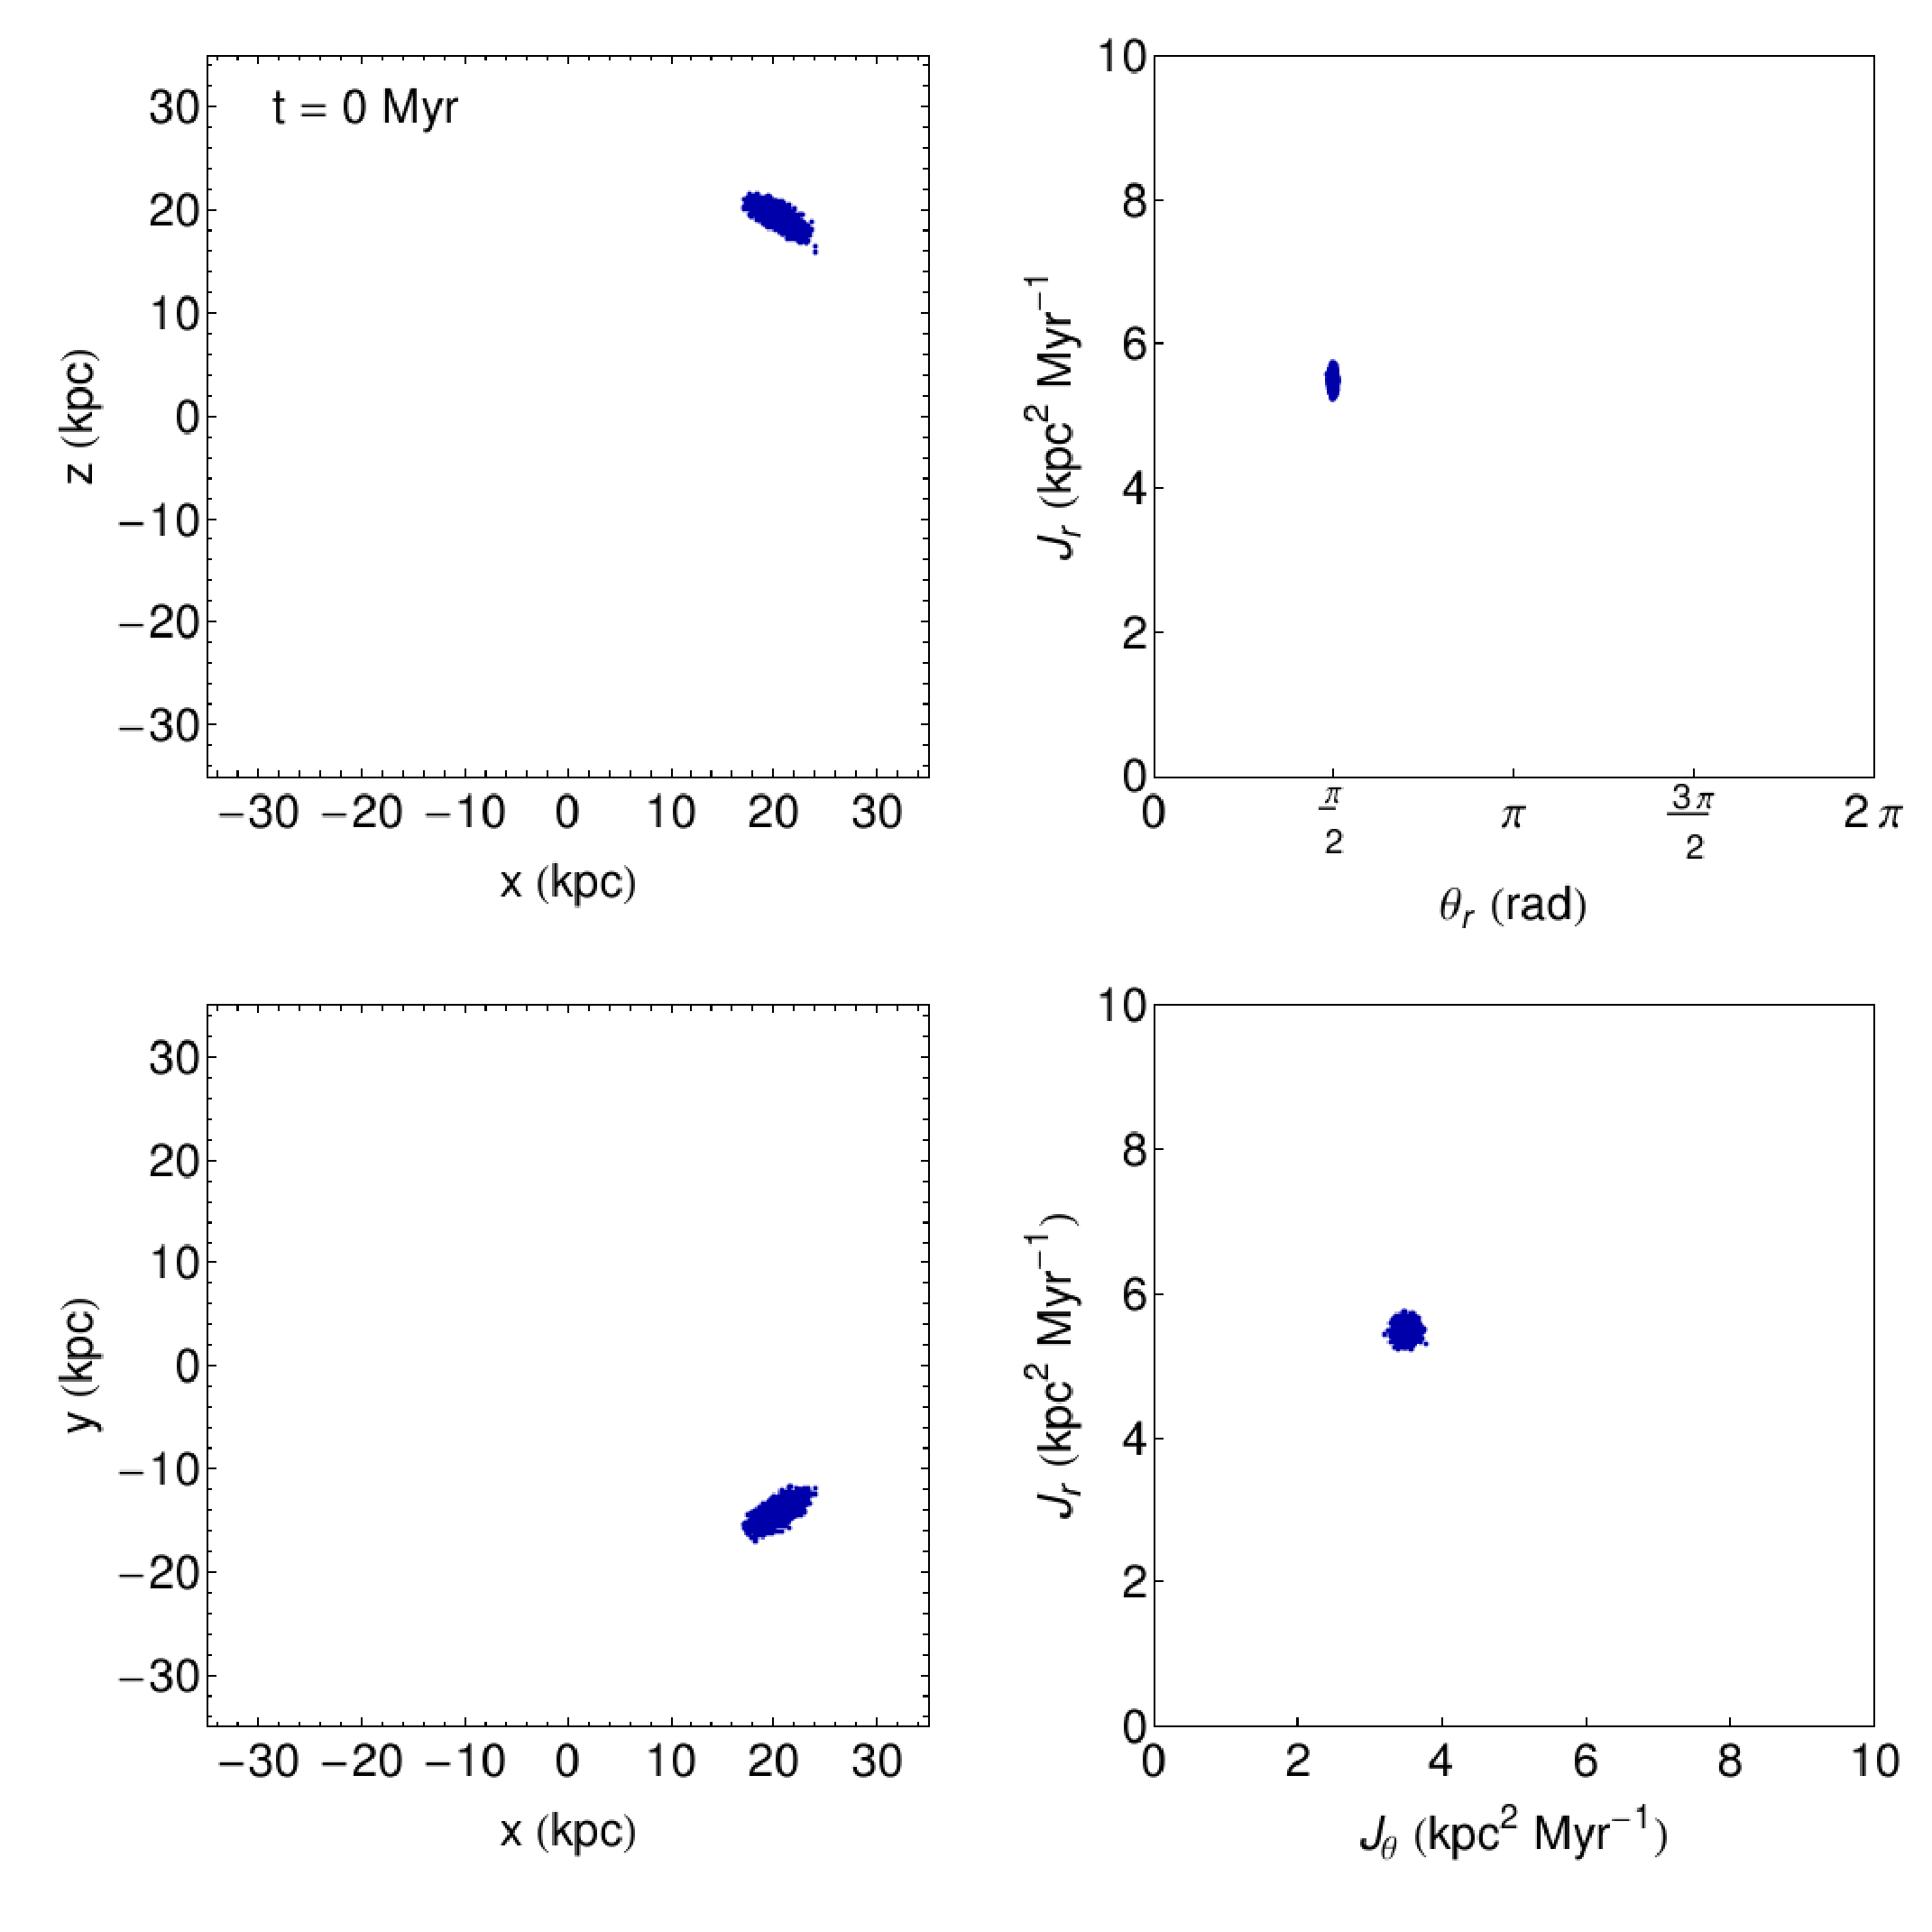
\includegraphics[width=1.6in]{Sanderson_Robyn_fig1_a.ps}  &
 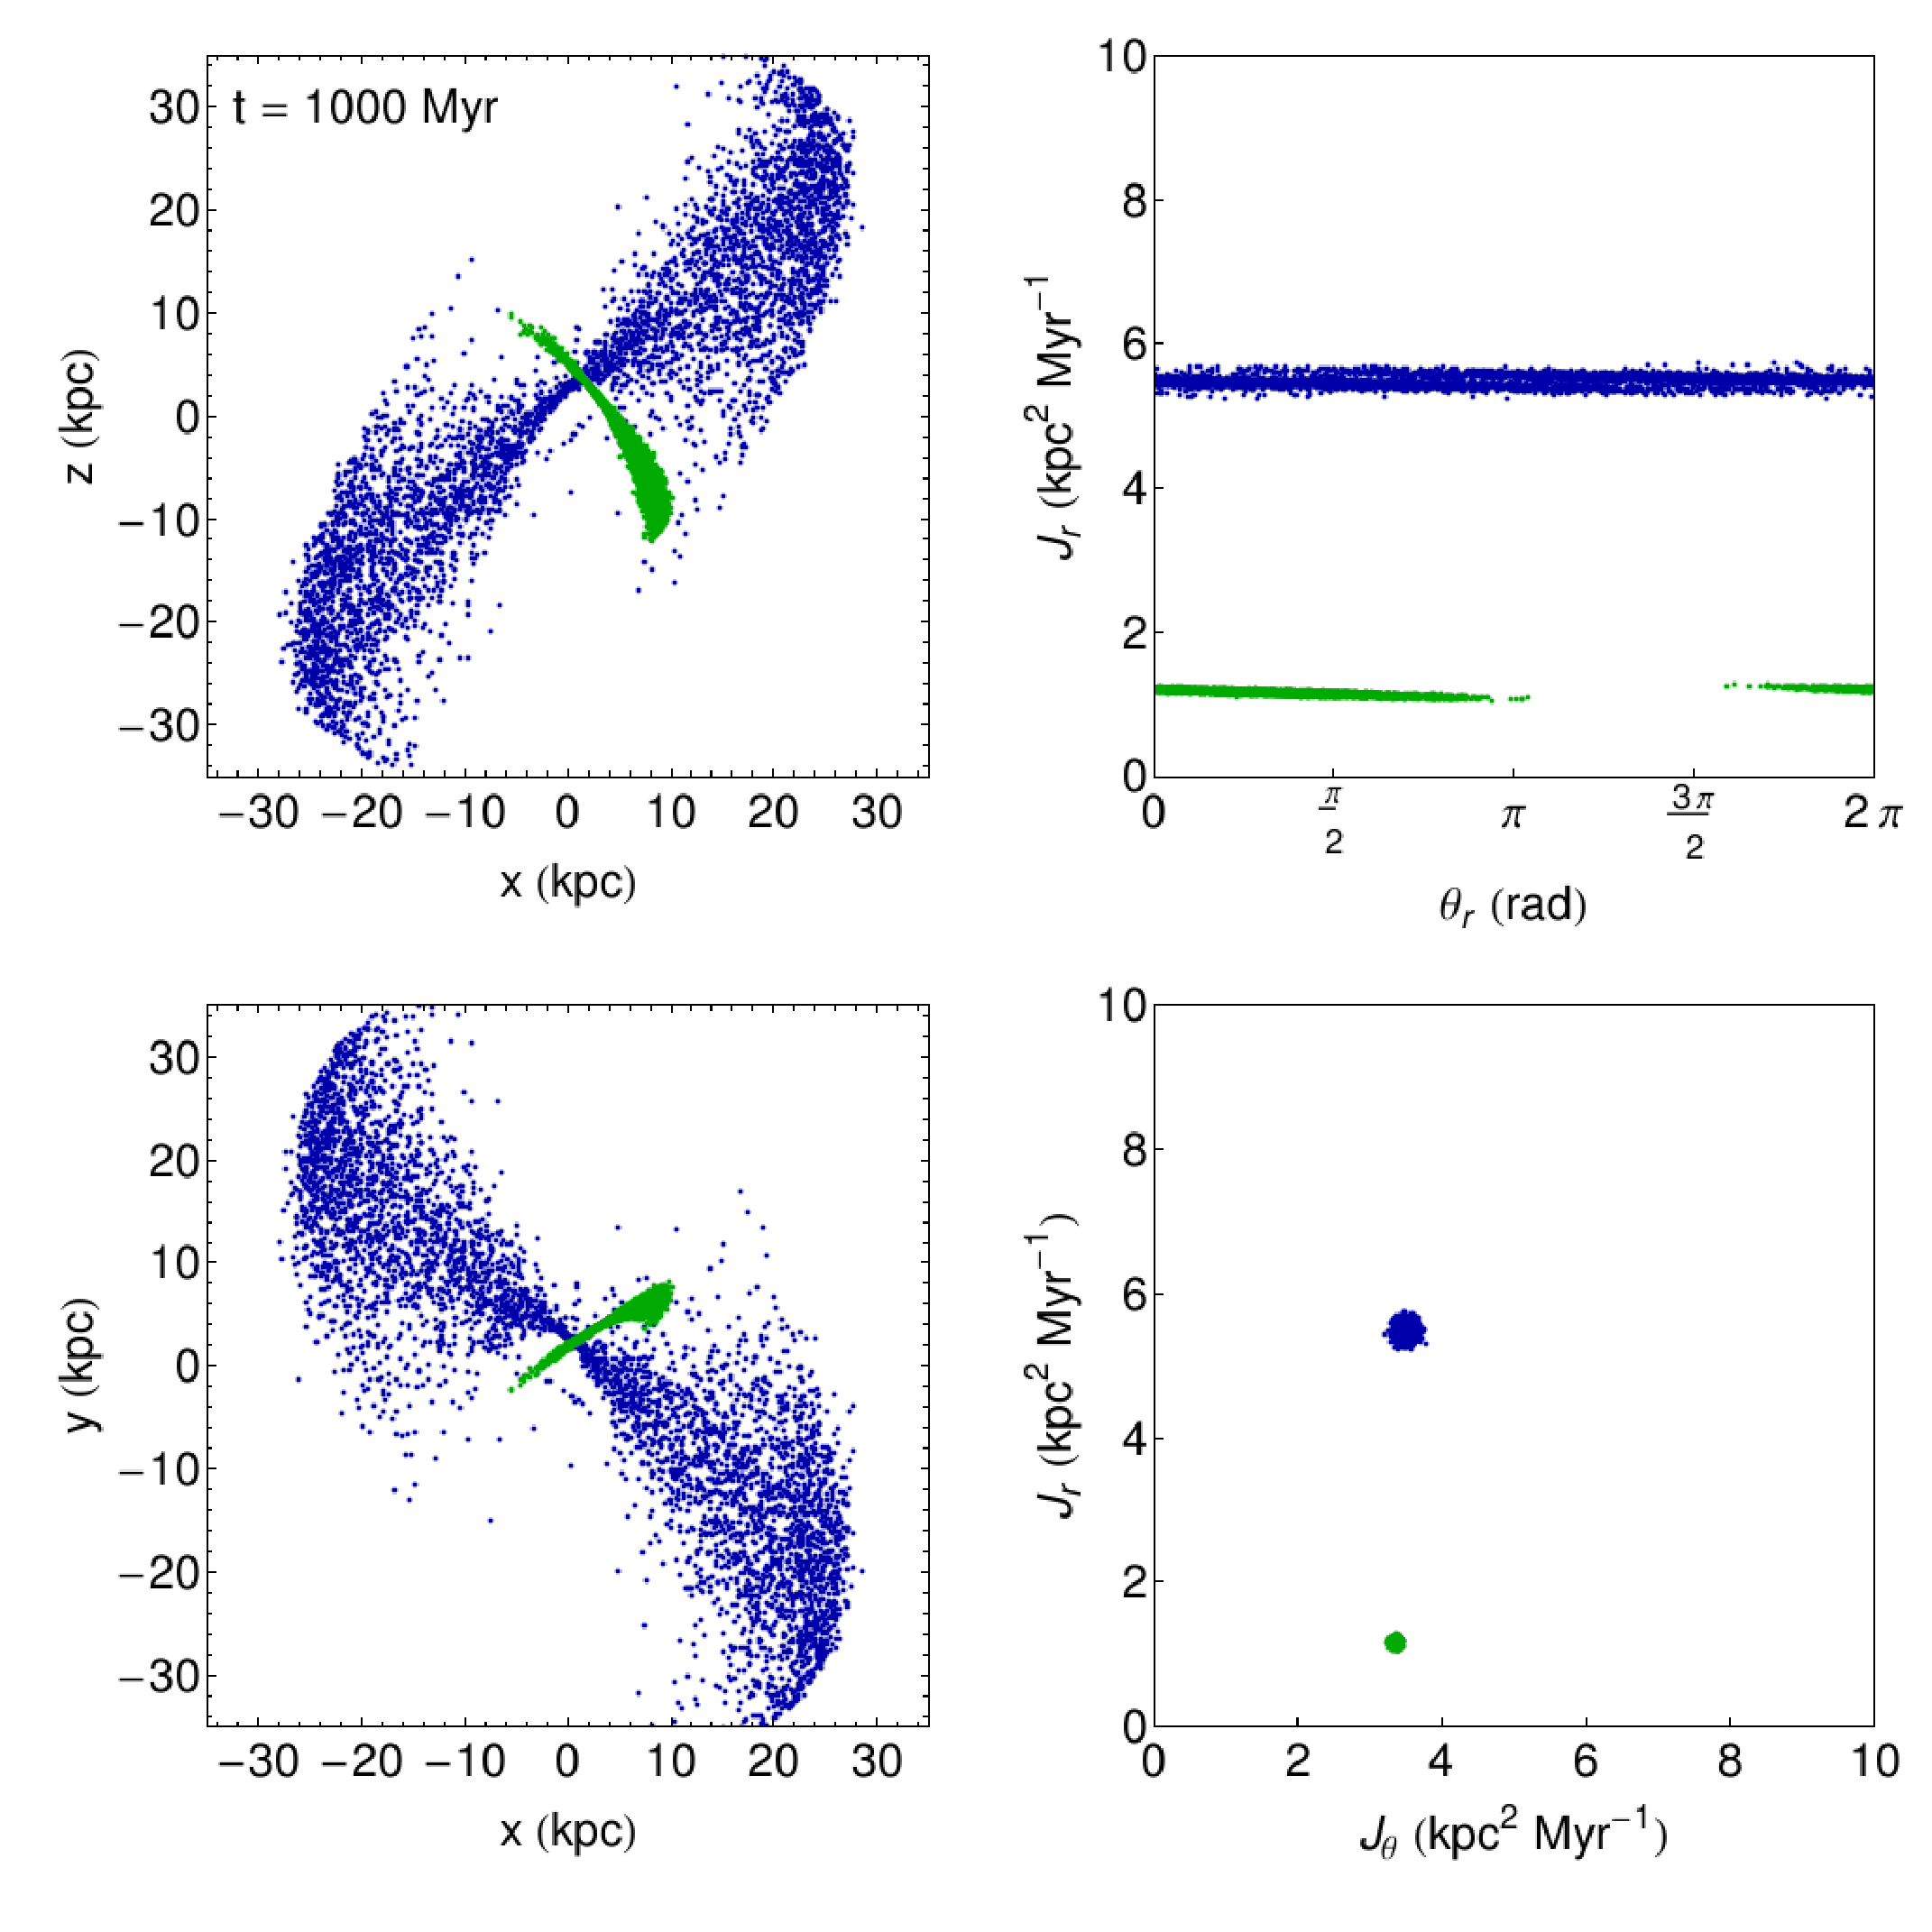
\includegraphics[width=1.6in]{Sanderson_Robyn_fig1_b.ps}  & 
  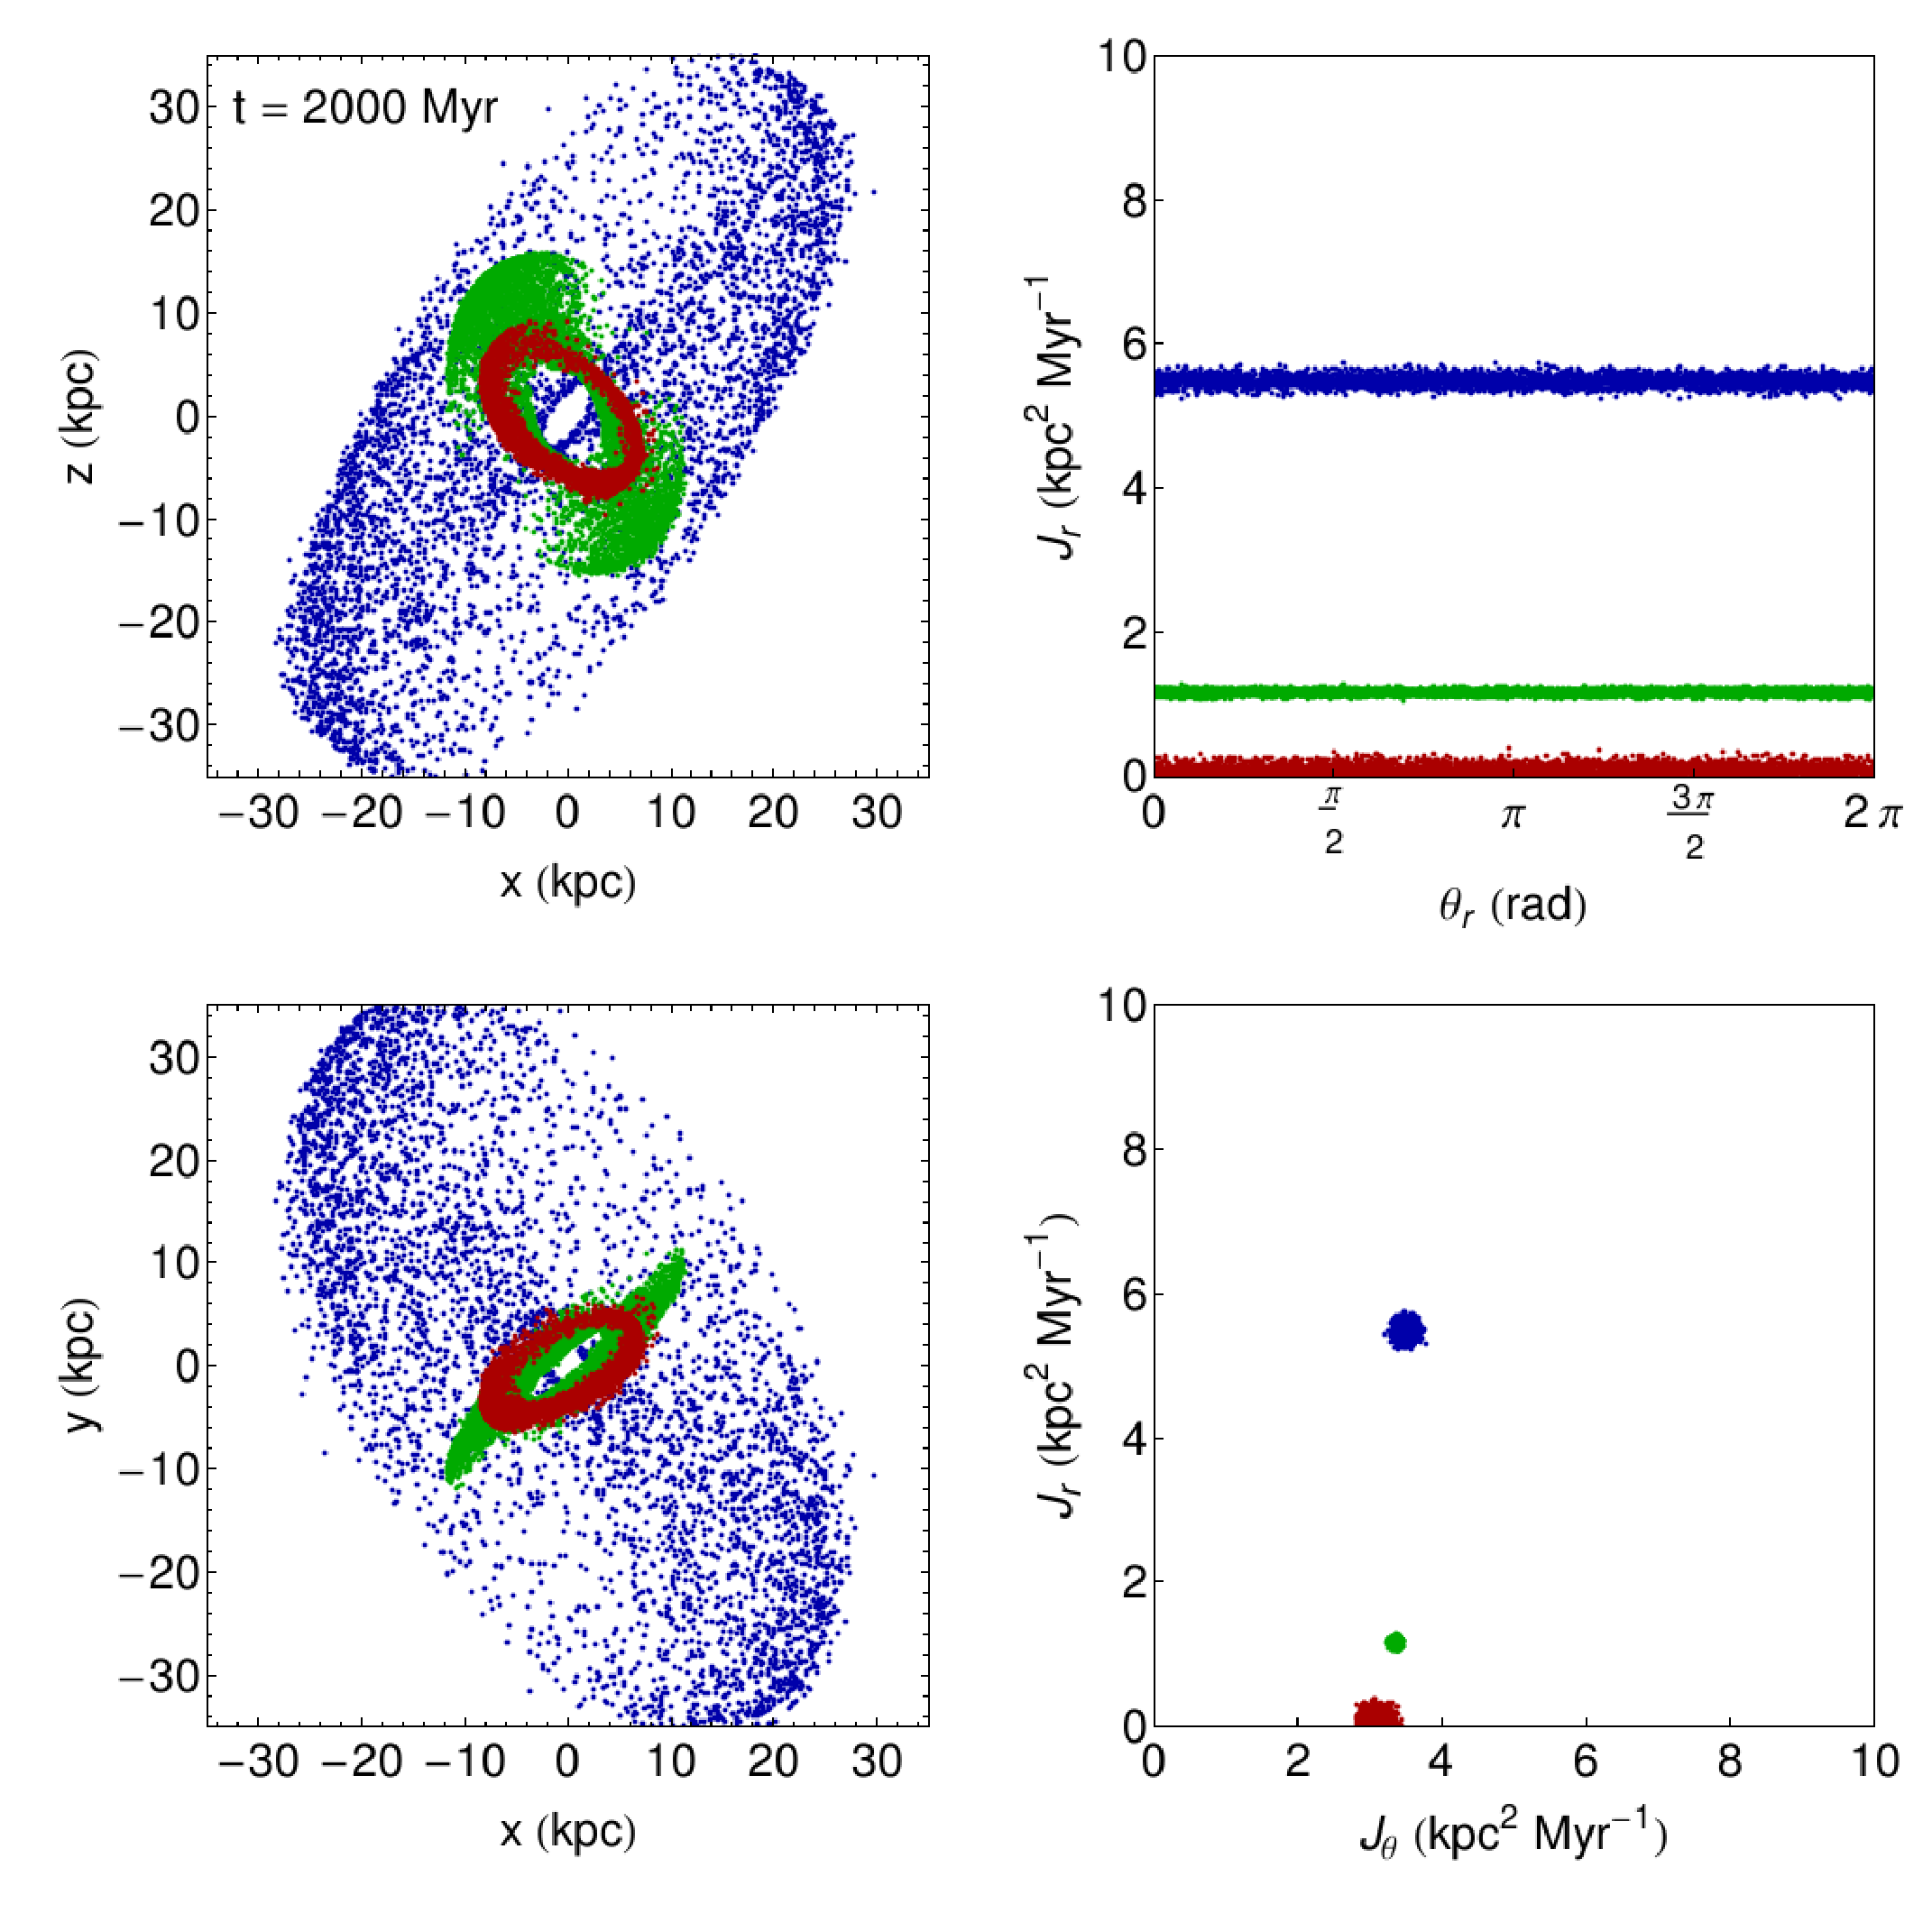
\includegraphics[width=1.6in]{Sanderson_Robyn_fig1_c.ps} 
\end{tabular} 
 % Plesae ensure all files are named according to instructions (see instructions to authors).
 \caption{Views of three tidal streams of different ages on different orbits in a static isochrone potential, shown at three different times: infall of the oldest stream (left), just after infall of the next-oldest stream (center), and after all three streams have evolved over many orbits (right). Over time the position distribution (left column) becomes complex and the angles (top right) become phase-mixed, but the action distribution (bottom right) remains clustered.  }
   \label{RES:fig1} % please use unique labels, such as your initials NNN:fig1
\end{center}
\end{figure}

This property of stream star actions implies that a statistical measure of the degree of clustering of the action distribution can be used as a merit function to find the best-fit gravitational potential. We use the Kullback-Leibler divergence \cite[KLD; Kullback \& Leibler 1951]{Kullback1951} for this purpose. For a continuous random variable $\mathbf{x}$, the KLD \emph{from} distribution $p(\mathbf{x})$ (e.g. the action distribution of the stream stars) \emph{to} a comparison distribution $q(\mathbf{x})$ (chosen so that it is guaranteed to be less clumpy that $p$) is defined as
\begin{equation}
 D_{KL}(p\to q) \equiv \int p(\mathbf{x}) \log \frac{p(\mathbf{x})}{q(\mathbf{x})} d\mathbf{x}.
\end{equation}
The KLD is not symmetric; it can be considered a measure of the relative entropy between $p$ and $q$. The lower the entropy (i.e., the higher the clustering) of $p$ relative to $q$, the higher the value of $D_{KL}$ (Figure \ref{RES:fig2}).

\begin{figure}[b]
\begin{center}
\begin{tabular}{cc}
 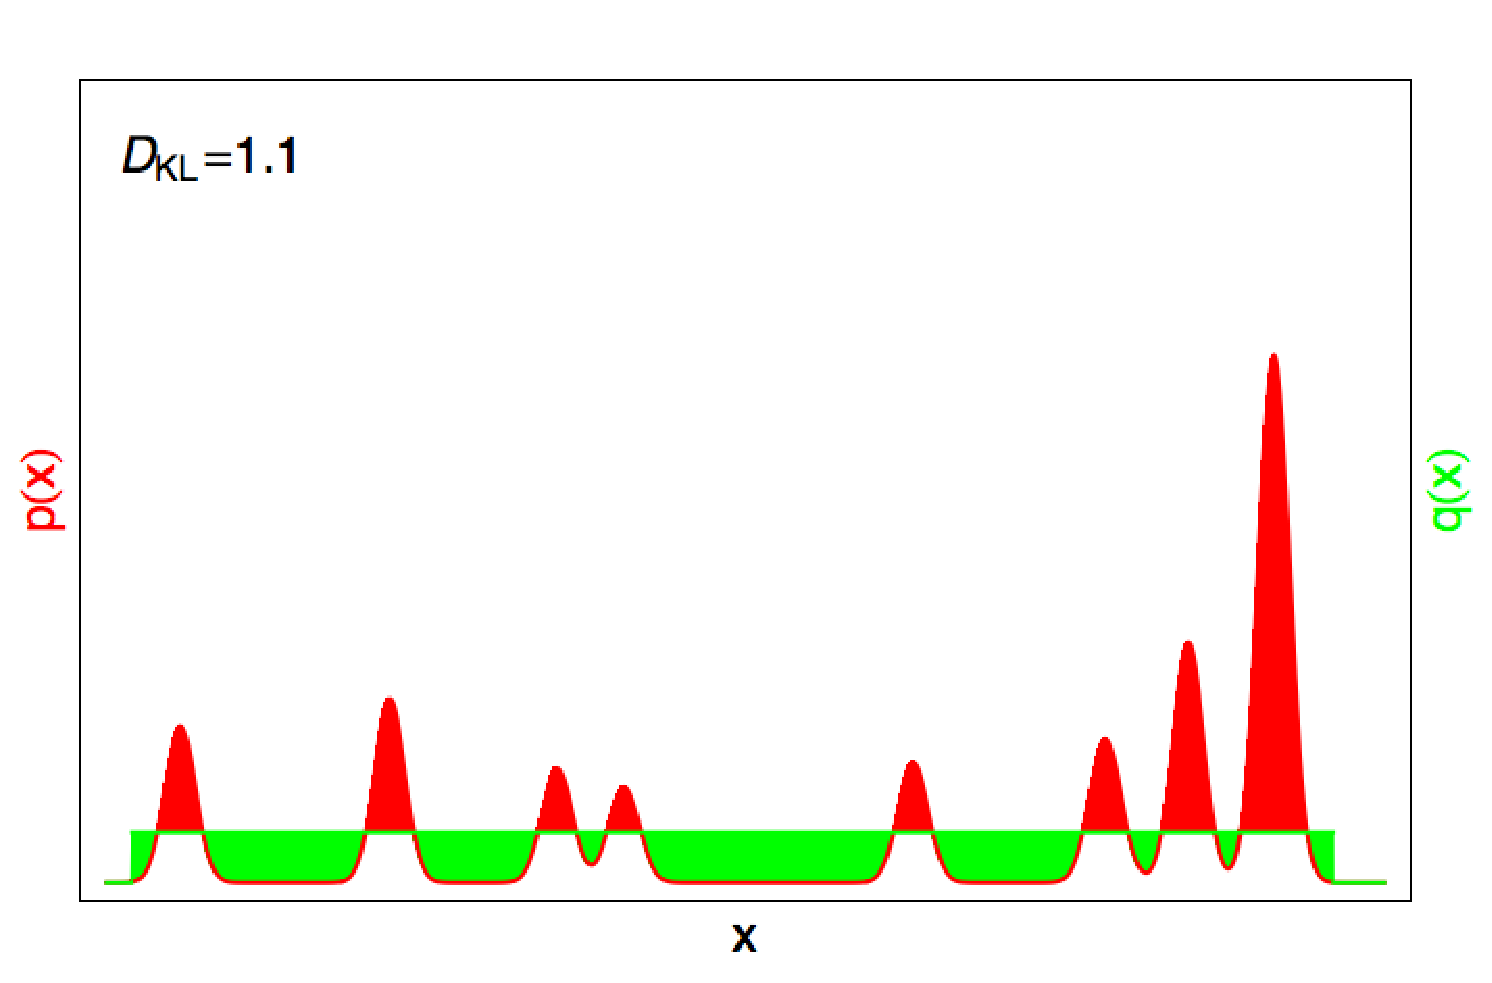
\includegraphics[width=2.4in]{Sanderson_Robyn_fig2_a.eps}  &
 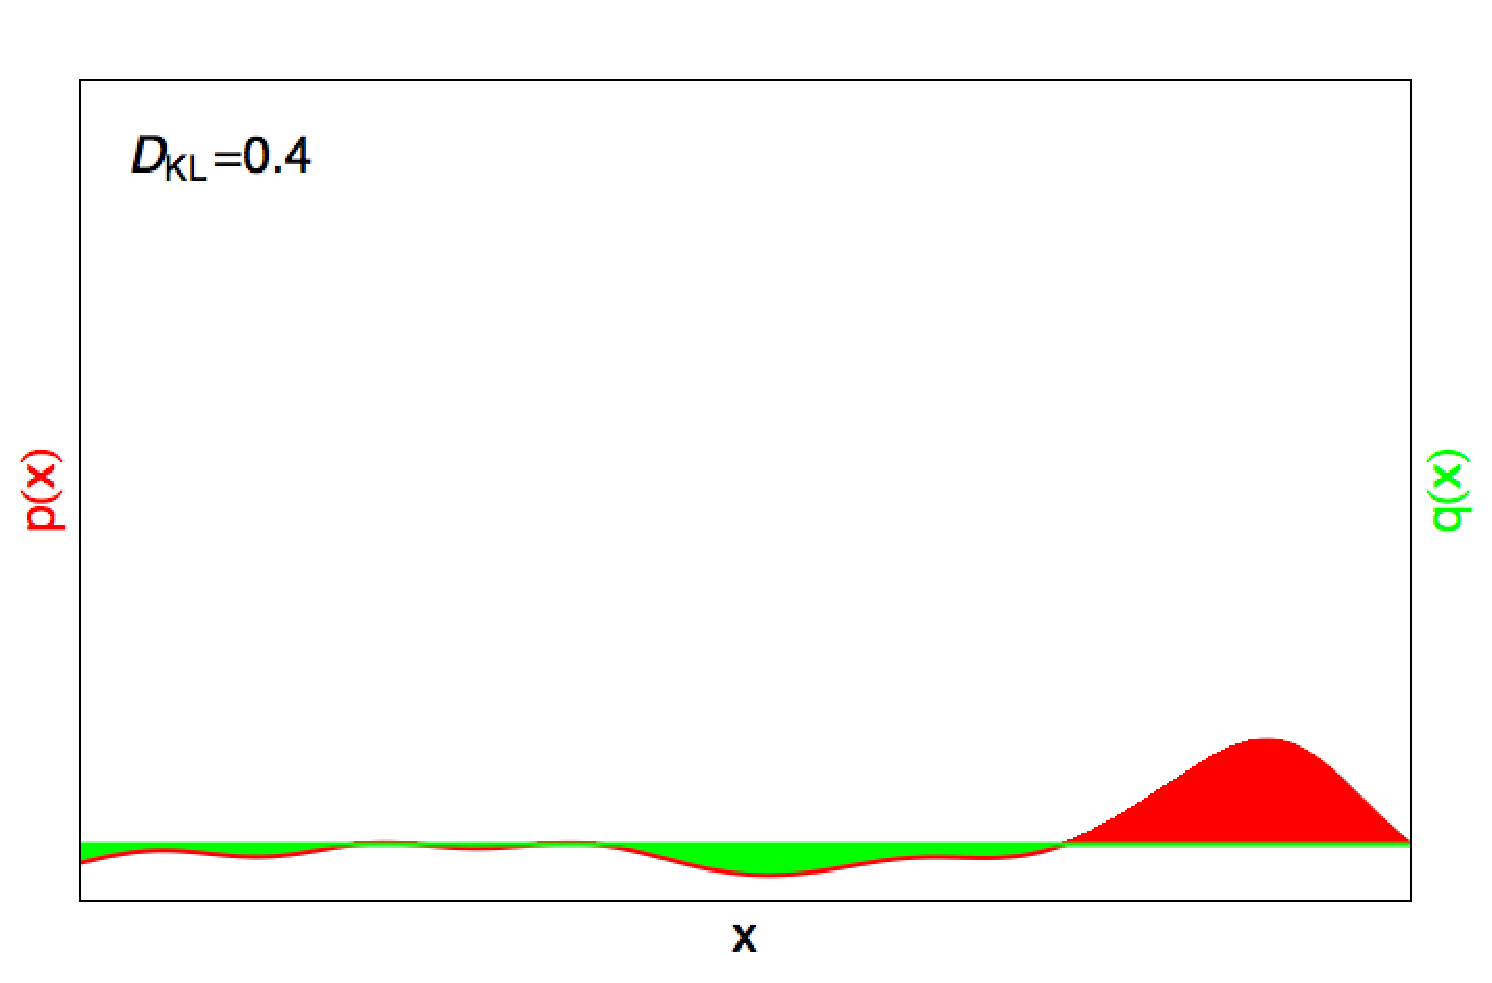
\includegraphics[width=2.4in]{Sanderson_Robyn_fig2_b.eps}   
\end{tabular} 
  \caption{}
   \label{RES:fig2} % please use unique labels, such as your initials NNN:fig1
\end{center}
\end{figure}
 
 \section{Construction of a mock Milky Way stellar halo}
 
 To test how well the KLD can recover the potential when used as a goodness-of-fit criterion, we constructed a mock Milky Way stellar halo by simulating the disruption of a set of satellite galaxies consistent with current expectations from observations and cosmological simulations. The galaxy luminosities were drawn from the measured luminosity function of Milky Way satellites given by \cite[Koposov et al. (2008)]{Koposov2008} and placed on the fundamental plane of \cite[Tollerud et al. (2011)]{Tollerud2011}. 
 
%%%%%%%%%%%%%%%%%%%%%%%%%%%%%%%%%%%%%%%%%%%%%%%%%%%
\begin{table}
  \begin{center}
  \caption{A table}
  \label{NNN:tab1}  % please use unique labels, such as your initials NNN:tab1
 {\scriptsize
  \begin{tabular}{lcccc}\hline 
{\bf Mineral} & {\bf Size [$\mu$m]} & {\bf Isotopic Signatures} & {\bf Stellar} & {\bf Contri-} \\ 
   &  {\bf abund.}  [ppm]$^1$ & & {\bf Sources} & {\bf bution$^2$} \\ \hline
diamond & $~0.0026$ & Kr-H, Xe-HL, Te-H & supernovae & ? \\
   & ~1500 & & & \\ \hline
silicon & $~0.1-10$ & enhanced $^{13}$C, $^{14}$N, $^{22}$Ne, s-process elem. & AGB stars & $> 90$~\% \\
carbide & $~30$ & low $^{12}$C/$^{13}$C, often enh.\ $^{15}$N & J-type C-stars (?) & $< 5$~\% \\
 & & enhanced $^{12}$C, $^{15}$N, $^{28}$Si; extinct $^{26}$Al, $^{44}$Ti & Supernovae & 1~\% \\
  \end{tabular}
  }
 \end{center}
\vspace{1mm}
 \scriptsize{
 {\it Notes:}\\
  $^1$For the abund.\ (in wt.\ ppm) the reported maximum values from different meteorites are given. \\
  $^2$Note uncertainty about actual fraction of diamonds that are pre-solar and for fraction of graphite attributed to SN and AGB stars (see discussion in text).}
\end{table}
%%%%%%%%%%%%%%%%%%%%%%%%%%%%%%%%%%%%%%%%%%%%%%%%%%%

\section{Implications}

{\underline{\it Grain formation}}. Chemical composition, sizes, and microstructures of grains constrain
conditions during condensation in stellar winds and supernova ejecta. Condensation of SiC
apparently occurred under close to the equilibrium conditions (e.g., 
\cite[Lodders \& Fegley 1998]{LoddersFegley98}).
Additional constraints are imposed by trace element contents both on average 
(\cite[Yin et al. 2006]{Yin_etal06}) 
as well as in individual grains 
(\cite[Amari et al. 1995]{Amari_etal95}). 
An important relevant observation is
the occurrence of subgrains of primarily TiC within graphite 
(\cite[Croat et al. 2005]{Croat_etal05}).

{\underline{\it The lifecycle of pre-solar grains (and maybe interstellar grains in general)}}. Interstellar grains
are expected to be processed and eventually destroyed by sputtering or astration (e.g.,
\cite[Draine 2003]{Draine03}), with an as yet unidentified process needed to account for the balance between
formation and destruction. Pre-solar grains preserved in meteorites carry, in principle, a
record of conditions they have been exposed to, which, however, is difficult to read.
Determining an absolute age using long-lived radioisotopes is virtually ruled out by the fact
that these systems use decay of rare constituents (e.g., K, Sr, Re, U) decaying into other rare
elements with uncertain non-radiogenic composition. However, appearance and
microstructures of pristine (i.e. not chemically processed) SiC show little evidence for being
processed, indicating either that they were surprisingly young when entering the forming
Solar System or that they were protected 
(\cite[Bernatowicz et al. 2003]{Bernatowicz_etal03}); a similar situation is
indicated by the lack of detectable spallation Xe produced by exposure to cosmic rays during residence in the ISM 
(\cite[Ott et al.  2005]{Ott_etal05}). The distribution, finally, among various types of
meteorites, provides a measure of processing in the early Solar System.

\bibliography{KLClusters}

%\bibitem[Amari \etal\ (1995)]{Amari_etal95}
%{Amari, S., Hoppe, P., Zinner, E., \& Lewis R.S.} 1995,
%\textit{Meteoritics}, 30, 490 


\begin{discussion}

{\it Please complete this section if questions have been collected during
your talk (and handed to you). Below are a couple of examples taken form 
an earlier proceeding. If no discusion took place and/or was not recorded
please delete the discussion section. Please note that the discssion must
fit inside the total number of allocated pages}

\discuss{Massey}{I�m wondering if you have considered the expected intrinsic dispersion in absolute
magnitude of WRs --� if you consider the (large) mass range that becomes an
early WN or late WC according to the evolutionary models, wouldn�t you expect a large
dispersion in M$_v$?}

\discuss{Your answer}{Indeed, we will be always left with some intrinsic scatter in M$_v$ due
to mass differences within the same spectral subtype. But in my opinion, the current
large dispersion is for a large fraction due to incertainties of the adopted distances of
open clusters and OB associations.}

\end{discussion}

\end{document}
